\documentclass{article}
\usepackage{graphicx}
\graphicspath{ {./images/} }
\usepackage{amsmath}
\usepackage{textcomp, gensymb}
\usepackage[export]{adjustbox}

\title{10. Kompleksie skaitļi - saknes vilkšana}
\author{Gunārs Ābeltiņš}
\date{2022-05-19}

\begin{document}

\maketitle

\section*{1. Uzdevums}
Aprēķiniet aptuveni visas vērtības 4.pakāpes saknei no skaitļa -4-3i, vispirms -  trigonometriskajā pierakstā, tad attēlojiet tās kompleksajā plaknē un iegūstiet ļoti aptuvenus algebriskos pierakstus.

\begin{equation*}
    |z| = \sqrt[2]{(-4)^2 + (-3)^2} = \sqrt{16 + 9} = \sqrt{25} = 5
\end{equation*}
\begin{equation*}
    \phi = - \arccos \frac{-4}{5} \approx - 140 \degree = 220 \degree
\end{equation*}
\begin{equation*}
    -4 - 3i = 5(\cos 220 \degree + i \sin 220 \degree)
\end{equation*}
\begin{equation*}
    \sqrt[4]{-4 - 3i} = \sqrt[4]{5}(\cos \frac{220 \degree + 360 \degree k}{4} + i \sin \frac{220 \degree + 360 \degree k}{4}) \approx
\end{equation*}
\begin{equation*}
    \approx 1.4(\cos (55 \degree + 90 \degree k) + i \sin (55 \degree + 90 \degree k))
\end{equation*}
\begin{equation*}
    k = 0 \Rightarrow 1.4 (\cos 55 \degree + \sin 55 \degree) \approx 0.8 + 1.1i
\end{equation*}
\begin{equation*}
    k = 1 \Rightarrow 1.4 (\cos 145 \degree + \sin 145 \degree) \approx -1.1 + 0.8i
\end{equation*}
\begin{equation*}
    k = 2 \Rightarrow 1.4 (\cos 235 \degree + \sin 235 \degree) \approx -0.8 - 1.1i
\end{equation*}
\begin{equation*}
    k = 3 \Rightarrow 1.4 (\cos 325 \degree + \sin 325 \degree) \approx 1.1 - 0.8i
\end{equation*}

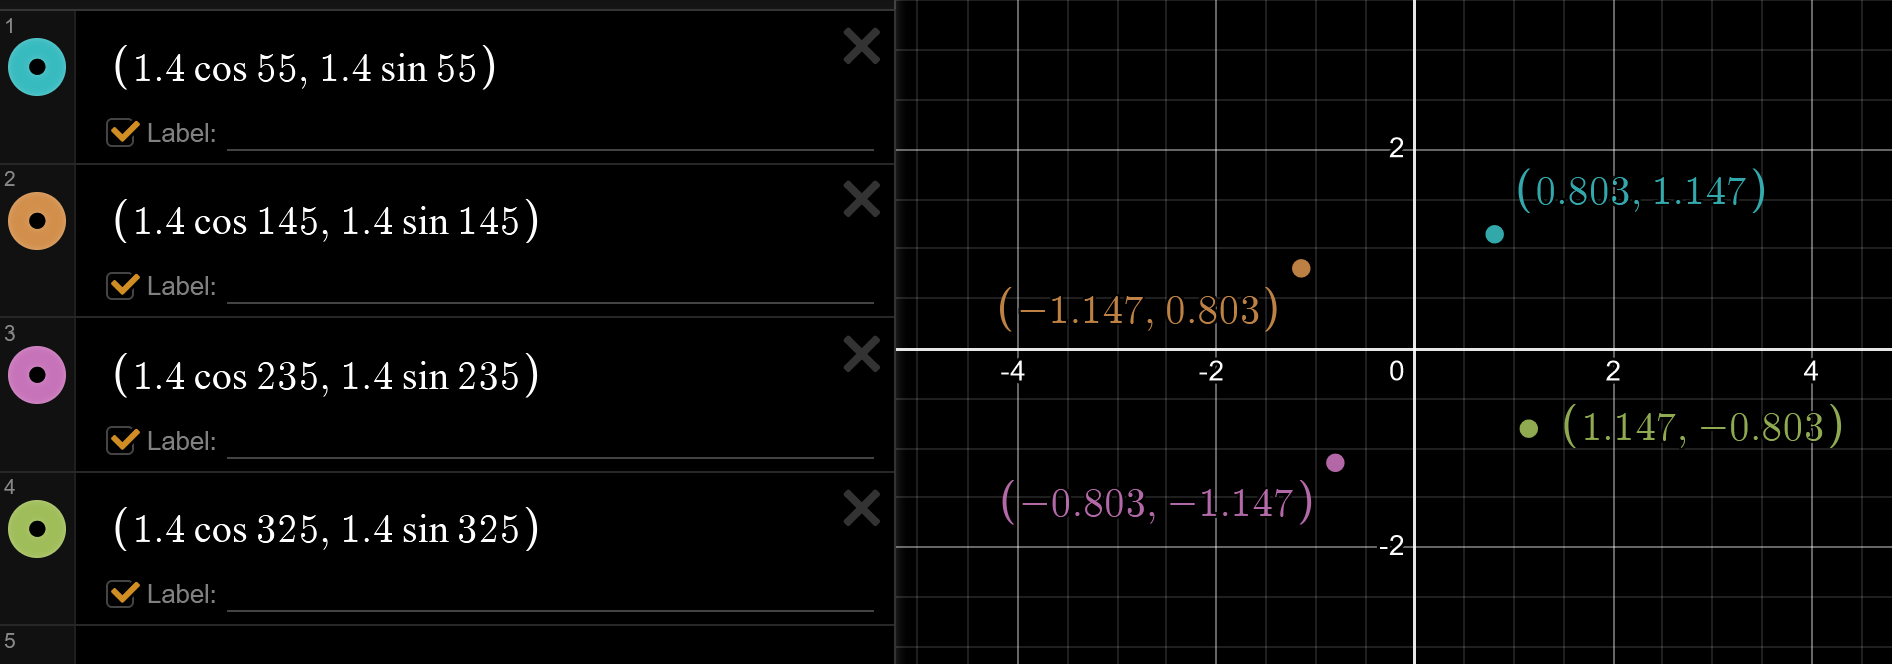
\includegraphics[width=0.9\textwidth, center]{1}

\section*{2. Uzdevums}
Aprēķiniet skaitļa z=(-17-6i)/(2-3i) algebrisko pierakstu, attēlojiet to kompleksajā plaknē un iegūstiet ļoti aptuvenu trigonometrisko pierakstu. Tad aprēķiniet visas vērtības kubsaknei no z, vispirms trigonometriskajā pierakstā, tad attēlojiet tās kompleksajā plaknē un iegūstiet ļoti aptuvenus algebriskos pierakstus.

\begin{equation*}
    z = \frac{-17 - 6i}{2 - 3i} = \frac{(-17 - 6i)(2 + 3i)}{(2 - 3i)(2 + 3i)} = \frac{-16 - 63i}{13} \approx -1.2 - 4.8i
\end{equation*}
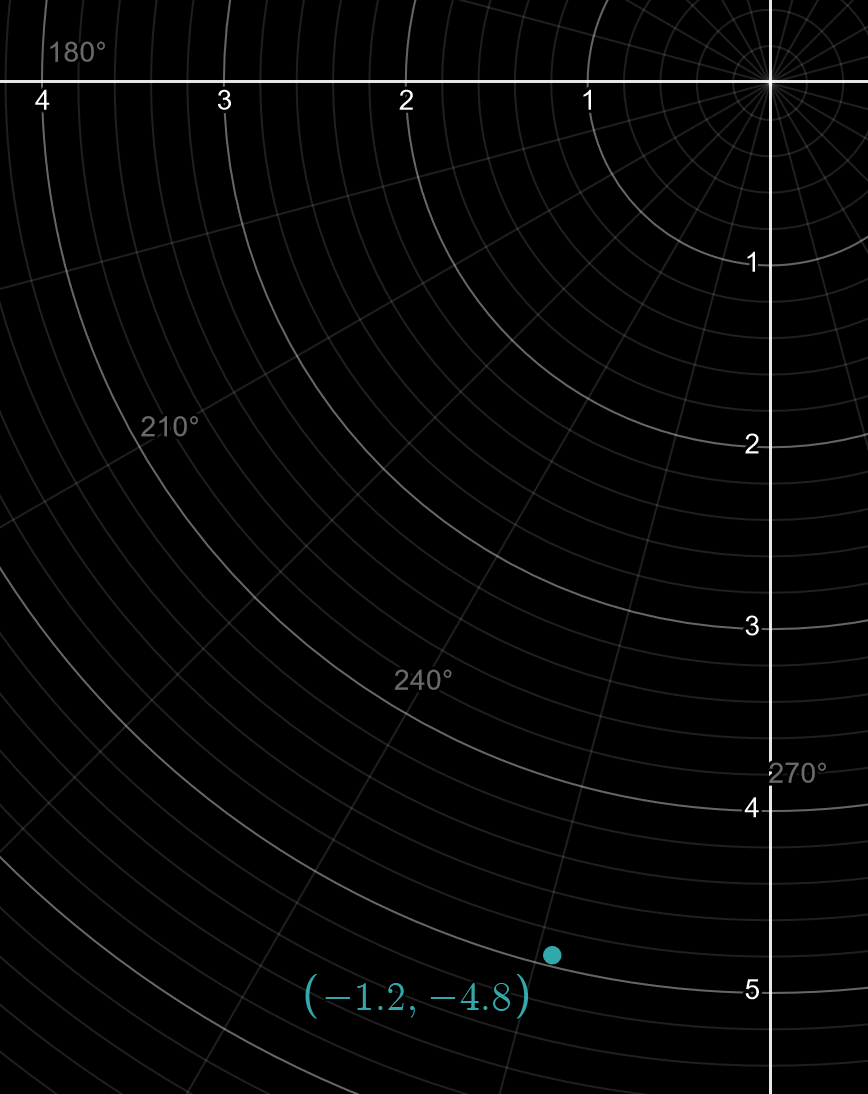
\includegraphics[width=0.9\textwidth, center]{2}
\begin{equation*}
    |z| = \sqrt[2]{(-1.2)^2 + (-4.8)^2} \approx 5
\end{equation*}
\begin{equation*}
    \phi = - \arccos \frac{-1.2}{5} \approx - 105 \degree = 255 \degree
\end{equation*}
\begin{equation*}
    z = 5(\cos 255 \degree + i \sin 255 \degree)
\end{equation*}
\begin{equation*}
    \sqrt[3]{z} = \sqrt[3]{5}(\cos \frac{255 \degree + 360 \degree k}{3} + i \sin \frac{255 \degree + 360 \degree k}{3}) \approx
\end{equation*}
\begin{equation*}
    \approx 1.7(\cos (85 \degree + 120 \degree k) + i \sin (85 \degree + 120 \degree k))
\end{equation*}
\begin{equation*}
    k = 0 \Rightarrow 1.7 (\cos 85 \degree + \sin 85 \degree) \approx 0.1 + 1.6i
\end{equation*}
\begin{equation*}
    k = 1 \Rightarrow 1.7 (\cos 205 \degree + \sin 205 \degree) \approx -1.5 + 0.7i
\end{equation*}
\begin{equation*}
    k = 2 \Rightarrow 1.7 (\cos 325 \degree + \sin 325 \degree) \approx 1.4 - 1.0i
\end{equation*}
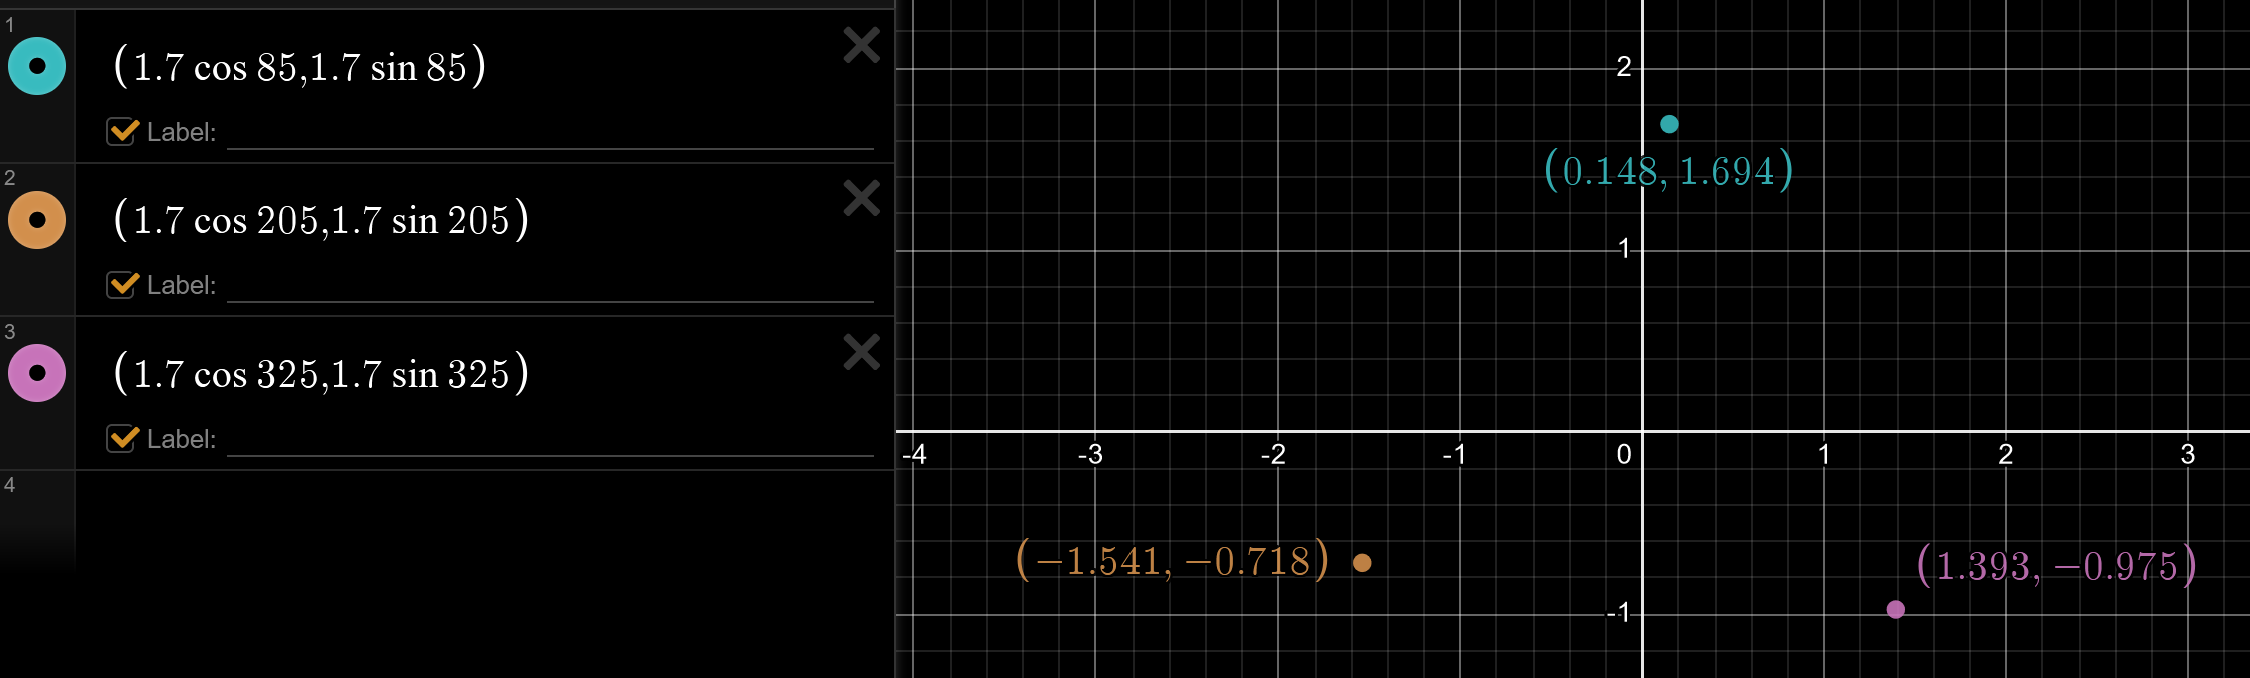
\includegraphics[width=0.9\textwidth, center]{3}

\section*{3. Uzdevums}
Aprēķiniet trigonometriskajā pierakstā visas vērtības 30-ās pakāpes saknei no skaitļiem 1 un i.

\begin{equation*}
    1 = 1(\cos 0 \degree + i \sin 0 \degree)
\end{equation*}
\begin{equation*}
    \sqrt[30]{1} = 1(\cos \frac{0 \degree + 360 \degree k}{30} + i \sin \frac{0 \degree + 360 \degree k}{30}) = \cos 12 \degree k + i \sin 12 \degree k
\end{equation*}
\begin{equation*}
    i = 1(\cos 90 \degree + i \sin 90 \degree)
\end{equation*}
\begin{equation*}
    \sqrt[30]{i} = 1(\cos \frac{90 \degree + 360 \degree k}{30} + i \sin \frac{90 \degree + 360 \degree k}{30}) = \cos (3 \degree + 12 \degree k) + i \sin (3 \degree + 12 \degree k)
\end{equation*}

\end{document}